% Created 2021-01-11 ma 10:15
% Intended LaTeX compiler: pdflatex
\documentclass[table]{beamer}

%%%% settings when exporting code %%%% 

\usepackage{listings}
\lstset{
backgroundcolor=\color{white},
basewidth={0.5em,0.4em},
basicstyle=\ttfamily\small,
breakatwhitespace=false,
breaklines=true,
columns=fullflexible,
commentstyle=\color[rgb]{0.5,0,0.5},
frame=single,
keepspaces=true,
keywordstyle=\color{black},
literate={~}{$\sim$}{1},
numbers=left,
numbersep=10pt,
numberstyle=\ttfamily\tiny\color{gray},
showspaces=false,
showstringspaces=false,
stepnumber=1,
stringstyle=\color[rgb]{0,.5,0},
tabsize=4,
xleftmargin=.23in,
emph={anova,apply,class,coef,colnames,colNames,colSums,dim,dcast,for,ggplot,head,if,ifelse,is.na,lapply,list.files,library,logLik,melt,plot,require,rowSums,sapply,setcolorder,setkey,str,summary,tapply},
emphstyle=\color{blue}
}

%%%% packages %%%%%

\usepackage[utf8]{inputenc}
\usepackage[T1]{fontenc}
\usepackage{lmodern}
\usepackage{textcomp}
\usepackage{color}
\usepackage{graphicx}
\usepackage{grffile}
\usepackage{wrapfig}
\usepackage{rotating}
\usepackage{longtable}
\usepackage{multirow}
\usepackage{multicol}
\usepackage{changes}
\usepackage{pdflscape}
\usepackage{geometry}
\usepackage[normalem]{ulem}
\usepackage{amssymb}
\usepackage{amsmath}
\usepackage{amsfonts}
\usepackage{dsfont}
\usepackage{array}
\usepackage{ifthen}
\usepackage{hyperref}
\usepackage{natbib}
\subtitle{}
\setbeamertemplate{footline}[frame number]
\setbeamertemplate{navigation symbols}{}
%
%%%% specifications %%%%
%
\usepackage{ifthen}
\usepackage{xifthen}
\usepackage{xargs}
\usepackage{xspace}
\newcommand\Rlogo{\textbf{\textsf{R}}\xspace} %
\RequirePackage{fancyvrb}
\DefineVerbatimEnvironment{verbatim}{Verbatim}{fontsize=\small,formatcom = {\color[rgb]{0.5,0,0}}}
\RequirePackage{enumitem}
\RequirePackage{colortbl} % arrayrulecolor to mix colors
\RequirePackage{pifont}
\RequirePackage{relsize}
\newcommand{\Cross}{{\raisebox{-0.5ex}%
{\relsize{1.5}\ding{56}}}\hspace{1pt} }
\newcommand{\Valid}{{\raisebox{-0.5ex}%
{\relsize{1.5}\ding{52}}}\hspace{1pt} }
\newcommand{\CrossR}{ \textcolor{red}{\Cross} }
\newcommand{\ValidV}{ \textcolor{green}{\Valid} }
\usepackage{stackengine}
\usepackage{scalerel}
\newcommand\Warning[1][3ex]{%
\renewcommand\stacktype{L}%
\scaleto{\stackon[1.3pt]{\color{red}$\triangle$}{\tiny\bfseries !}}{#1}%
\xspace
}
\usepackage{changepage}
\usepackage{booktabs}
\newcommand{\darkgreen}{green!50!black}
\RequirePackage{epstopdf} % to be able to convert .eps to .pdf image files
\RequirePackage{capt-of} %
\RequirePackage{caption} % newlines in graphics
\newcommand{\backupbegin}{
\newcounter{finalframe}
\setcounter{finalframe}{\value{framenumber}}
}
\newcommand{\backupend}{
\setcounter{framenumber}{\value{finalframe}}
}
\RequirePackage{hanging}
\setbeamertemplate{footnote}{%
\hangpara{2em}{1}%
\makebox[2em][l]{\insertfootnotemark}\footnotesize\insertfootnotetext\par%
}
\usetheme[height=20pt]{Singapore}
\author{Brice Ozenne}
\date{\today}
\title{"How to" in orgmode}
\hypersetup{
 colorlinks=true,
 citecolor=[rgb]{0,0.5,0},
 urlcolor=[rgb]{0,0,0.5},
 linkcolor=[rgb]{0,0,0.5},
 pdfauthor={Brice Ozenne},
 pdftitle={"How to" in orgmode},
 pdfkeywords={},
 pdfsubject={},
 pdfcreator={Emacs 25.2.1 (Org mode 9.0.4)},
 pdflang={English}
 }
\begin{document}

\maketitle

\section{Box}
\label{sec:org156da8b}

\begin{frame}[label={sec:org767f7f4}]{Round box}
\setbeamercolor{block title example}{fg=black,bg=lightgray}
\setbeamercolor{block body example}{fg=white,bg=gray}
\setbeamercolor{block body}{fg=white,bg=blue!60}

\begin{block}{}
	The \texttt{beamercolorbox} environment!
\end{block}

\begin{exampleblock}{block title}
	Box type \texttt{beamerboxesrounded}
	
	with shadow.
	
	Different colours are possible for the header and box contents. \ldots
\end{exampleblock}

\setbeamertemplate{blocks}[rounded][shadow=true]
\begin{example}
	Box type \texttt{beamerboxesrounded}
	
	with shadow.
	
	Different colours are possible for the header and box contents. \ldots
\end{example}
\end{frame}

\section{Code}
\label{sec:orga6b8914}

\begin{frame}[fragile,label={sec:orga89559e}]{Set output size}
 \lstset{language=r,label= ,caption= ,captionpos=b,numbers=none}
\begin{lstlisting}
summary(model)
\end{lstlisting}


{
\RecustomVerbatimEnvironment{verbatim}{Verbatim}{fontsize=\scriptsize,formatcom = {\color[rgb]{0.5,0,0}}}

\begin{verbatim}
________________________________________________________________________________
Layer (type)                        Output Shape                    Param #     
================================================================================
dense_22 (Dense)                    (None, 256)                     200960      
________________________________________________________________________________
dense_23 (Dense)                    (None, 128)                     32896       
________________________________________________________________________________
dense_24 (Dense)                    (None, 10)                      1290        
================================================================================
Total params: 235,146
Trainable params: 235,146
Non-trainable params: 0
________________________________________________________________________________
\end{verbatim}

}

\lstset{language=r,label= ,caption= ,captionpos=b,numbers=none}
\begin{lstlisting}
model$weights[[1]]
\end{lstlisting}

{
\RecustomVerbatimEnvironment{verbatim}{Verbatim}{fontsize=\scriptsize,formatcom = {\color[rgb]{0.5,0,0}}}

\begin{verbatim}
<tf.Variable 'dense_4/kernel:0' shape=(784, 256) dtype=float32_ref>
\end{verbatim}

}
\end{frame}

\section{List}
\label{sec:org8976527}

\begin{frame}[label={sec:orgd0eb3ee}]{Choose item}
\begin{description}
\item[{(A)}] yyy
\item[{(1)}] xxx
\end{description}
\end{frame}

\begin{frame}[label={sec:orge5a2da2}]{Use itemize and modify vertical space}
\begin{itemize}[label={-},topsep=0pt,itemsep=0mm]
\item a
\item b
\item c
\end{itemize}
\end{frame}

\begin{frame}[label={sec:org5af868c}]{label scheme}
\begin{itemize}
\item level 1: \textbullet
\item level 2: \textendash
\item level 3: \textasteriskcentered
\item level 4: \textperiodcentered
\end{itemize}
\end{frame}
\section{Table}
\label{sec:org13a8a2a}

\begin{frame}[label={sec:org6089f3c}]{Nice latex table}
(require booktabs)

\begin{table}
\begin{tabular}{lll}
\toprule
A  & \textcolor{orange}{B} & \textcolor{blue}{C} \\
D & (n=282)  & (n=280) \\
\midrule
Grade 1 & 48 (17\%)  & 69 (24.6\%) \\
Grade 2 & 118 (41.8\%)  & 89 (31.5\%) \\
Grade 3 & 72 (25.5\%)  & 47 (16.8\%) \\
Grade 4 & 11 (3.9\%) & 6 (2.1\%) \\
Grade 5 & 4 (1.4\%)  & 3 (1.1\%) \\
\bottomrule
\end{tabular}
\end{table}
\end{frame}

\section{References}
\label{sec:orgc42459c}

\begin{frame}[label={sec:org4bb4aac}]{Citations}
\begin{itemize}
\item \citep{pearson1905problem}
\item \cite{pearson1905problem}
\item \citep[xx]{pearson1905problem}
\end{itemize}
\cite[p.~150]{pearson1905problem}
\end{frame}

\section{Miscellaneous}
\label{sec:org078015f}

\begin{frame}[label={sec:orgfb15cf2}]{Divide the page (align at the middle)}
\begin{columns}
\begin{column}{0.45\columnwidth}
\begin{itemize}
\item topic
\begin{itemize}
\item subtopic
\item sub
\end{itemize}
\item topic
\end{itemize}
\end{column}

\begin{column}{0.45\columnwidth}
\begin{center}
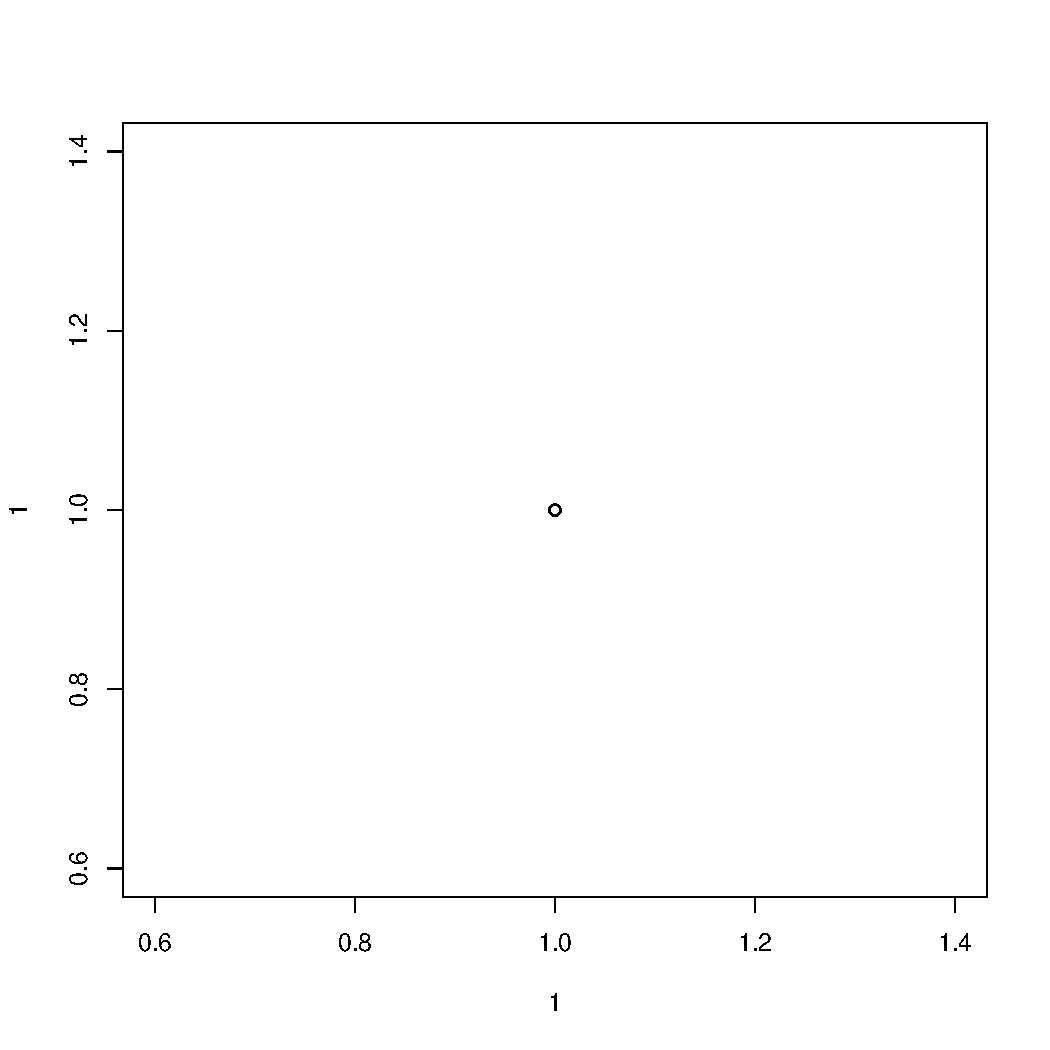
\includegraphics[width=.9\linewidth]{./figures/myplot.pdf}
\end{center}
\end{column}
\end{columns}
\end{frame}

\begin{frame}[label={sec:org4415a14}]{Divide the page (align at the top)}
\begin{columns}
\begin{column}[t]{0.45\columnwidth}
\begin{itemize}
\item topic
\begin{itemize}
\item subtopic
\item sub
\end{itemize}
\item topic
\end{itemize}
\end{column}

\begin{column}[T]{0.45\columnwidth}
\begin{center}
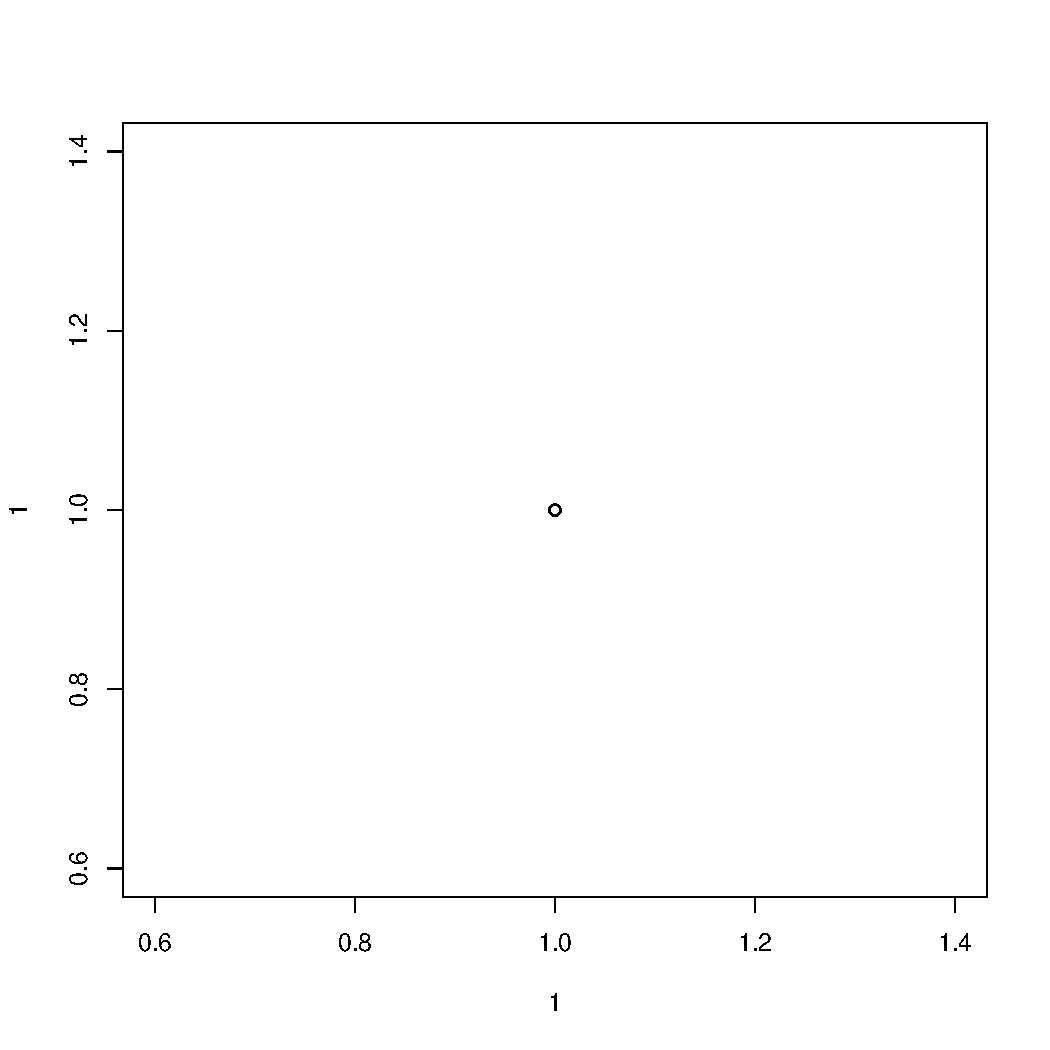
\includegraphics[width=.9\linewidth]{./figures/myplot.pdf}
\end{center}
\end{column}
\end{columns}
\end{frame}

\begin{frame}[label={sec:org36f7989}]{Inline latex}
any arbitrary LaTeX code
\end{frame}

\begin{frame}[label={sec:orgea022dc}]{Color tex}
(see header for the definition of darkgreen)
\begin{itemize}
\item \textcolor{\darkgreen}{risk factor}: adjust (will increase precision)
\end{itemize}
\end{frame}

\begin{frame}[label={sec:org68ccc58}]{Footnote}
This is a footnote\footnote{blaa}.
\end{frame}
\begin{frame}[label={sec:org2c7c5be}]{Big centered text}
\vfill

\begin{center}
\Huge Quiz
\end{center}

\vfill
\end{frame}

\begin{frame}[label={sec:org4cdf08a}]{Change margin}
(require changepage)
\begin{adjustwidth}{-1em}{-1em}
xxxxxxxxxxxxxxxxxxxxxxxxxxxxxxxxxxxxxxxxxxxxxx
\end{adjustwidth}
\begin{adjustwidth}{-3em}{-3em}
xxxxxxxxxxxxxxxxxxxxxxxxxxxxxxxxxxxxxxxxxxxxxx
\end{adjustwidth}
\end{frame}

\begin{frame}[label={sec:org460afee}]{Comments}
\end{frame}
\section{References}
\label{sec:org28f3c79}
\begingroup
\renewcommand{\section}[2]{}
\bibliographystyle{apalike}
\bibliography{bibliography}

\endgroup
\end{document}